\section{Техническое задание}
\subsection{Основание для разработки}

Основанием для разработки является задание на выпускную квалификационную работу бакалавра "<Интеллектуальная система распознавания объектов по цветовым характеристикам на основе нечетких нейронных сетей">.

\subsection{Цель и назначение разработки}

Основной задачей выпускной квалификационной работы является разработка интеллектуальной системы распознавания объектов на основе их цветовых характеристик с использованием нечетких нейронных сетей. Система должна обеспечивать высокую точность распознавания объектов различных классов на основе их цветовых параметров.

Задачами данной разработки являются:
\begin{itemize}
\item сбор набора данных, содержащего изображения объектов различных классов;
\item предварительная обработка изображений для выделения цветовых характеристик объектов;
\item проектирование архитектуры нечеткой нейронной сети;
\item обучение нейронной сети на подготовленных данных;
\item создание удобного поиска по сайту;
\item оптимизация параметров сети для достижения максимальной точности распознавания;
\item создание программного интерфейса для взаимодействия с разработанной нейронной сетью.
\end{itemize}

\subsection{Требования пользователя к интерфейсу приложения}

Приложение должно включать в себя:
\begin{itemize}
    \item графический интерфейс пользователя;
    \item возможность загрузки изображений объектов для их распознавания;
    \item отображение результатов распознавания с указанием класса объекта и уверенности в распознавании;
    \item возможность обучения системы на пользовательских данных для улучшения качества распознавания;
    \item интерфейс для добавления новых классов объектов и их обучения;
    \item возможность экспорта результатов распознавания в формате, подходящем для дальнейшей обработки или анализа.
\end{itemize}

Композиция шаблона приложения представлена на рисунке ~\ref{maket:image}.

\begin{figure}[ht]
\includegraphics[width=1\linewidth]{maket}
\caption{Композиция шаблона приложения}
\label{maket:image}
\end{figure}
%\vspace{-\figureaboveskip} % двойной отступ не нужен (можно использовать, если раздел заканчивается картинкой)

\subsection{Моделирование вариантов использования}

Для моделирования вариантов использования разрабатываемого приложения была использована диаграмма вариантов использования, представленная на рисунке ~\ref{usecase:image}.

\begin{figure}[ht]
\centering
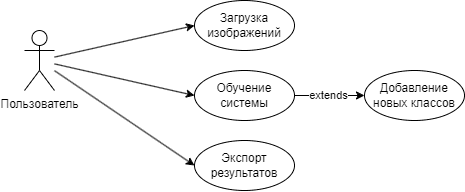
\includegraphics[width=0.8\linewidth]{usecase}
\caption{Диаграмма вариантов использования}
\label{usecase:image}
\end{figure}

На диаграмме представлены основные варианты использования приложения, включая загрузку изображений для распознавания, обучение системы, добавление новых классов объектов и экспорт результатов распознавания. Данная диаграмма помогает понять основные функциональные возможности приложения и взаимодействие с пользователями.

На основании анализа предметной области в программе должны быть реализованы следующие прецеденты:
\begin{enumerate}
\item Распознание объекта на изображении по его цветовым характеристикам;
\item Сохранение результатов распознания для дальнейшего использования;
\item Обучение и переобучение нейро-нечёткой сети;
\item Сохранение результатов обучения для дальнейшего расспознания.
\end{enumerate}

\subsection{Требования к оформлению документации}

Разработка программной документации и программного изделия должна производиться согласно ГОСТ 19.102-77 и ГОСТ 34.601-90. Единая система программной документации.
